\chapter{Distance education}

Distance education is not only a phenomenon of the last few decades, but can be traced at least back to the 18th century, when Caleb Phillipps posted an advertisment called ``Teacher of the New Method of Short Hand'' in Boston Gazette, saying ``Persons in the Country desirous to Learn this Art, may by having the several Lessons sent weekly to them, be as perfectly instructed as those that live in Boston.''~\cite{1}

With the development of the Internet and its general accessibility in the developed world, providing distance education has become much easier and has spread widely. In some countries tuition rates are high and young people take loans so they can affoard to study. This topic is covered in a fitting way by John Oliver in his show~\cite{2}. The flexibility and low cost of distance education over the Internet gives people, who wouldn't be otherwise able to attend a traditional university, an opportunity to gain knowledge and train skills from their homes~\cite{3} spending much less money or even for free.

Students in the developing world are also taking the advantage of educational content available on the Internet. Several of the top U.S. universities, like Harvard, Stanford or MIT, put some of their materials on so called \textit{Massive Open Online Courses} (MOOC) \nomenclature{MOOC}{Massive Open Online Course} like Coursera, edX or Udacity. This content is then available to anyone with a computer and Internet connection and knowledge of the language. A great example is \textit{Kepler} - a non profit university project in Rwanda~\cite{5}. The goal of this project is to ``provide an American-accredited degree, a world class education, and a clear path to good jobs for thousands of students for around \$1,000 tuition per year.''~\cite{6}

A concept of teaching often reffered to as \textit{Flipped Classroom} uses distance education. The idea is to let students study lecture materials at home at their own pace and then apply gained knowledge at school the next day by doing activities to illustrate the concepts. The teacher can then help them or explain details in person. These materials are often in the form of videos either from an open source, like the Khan Academy, or created by the teachers themselves.

\section{Current systems}
In the next few paragraphs I will try to pick some of current distance education services and tools available on the Internet. This list is not complete and is only meant to give the reader a notion of available technologies and their paradigms, on which the project of Vector Screencast is based.

\subsection{Coursera}
The mission of \textit{Coursera} is to ``provide universal access to the world’s best education.''\cite{9} Anyone can, for free, go through materials published by universities and other organizations aimed at education.

Courses at Coursera consist mainly of video lectures commonly with a transcript and an  attached presentation document. These videos can be viewed directly in web browser on demand or downloaded to user's computer. After studying the materials, students can submit assignments' solutions and take quizzes and receive a Verified Certificate for the accomplishment of the course. These certificates are not for free.

Most of the courses are in English and only a few of the courses are also translated into other languages. It is not possible for everyone to publish his materials through Coursera.



\subsection{Youtube.com}
\textit{Youtube.com}~\cite{10} is not an educational service by design. Youtube allows people to create their own channels and upload their video content to share it with other Internet users for free.

Youtube was launched in 2005 and has became one of the most frequently visited websites on the Internet according to Alexa Internet~\cite{11}. Uploading video to Youtube is free, advertisment is displayed to the user while watching videos though.

The ease of making original-created videos available for wide audience makes Youtube a perfect place for all individuals and organizations, who want to share their ideas or any video materials. Many educational channels can be found here, for example \textit{Numberphile}~\cite{numberphile_youtube}, \textit{Veritasium}~\cite{veritasium_youtube}, and \textit{Khan Academy}~\cite{khan_academy_youtube}.

Youtube videos can be viewed only online in a web browser or a specialized mobile app. There are only unofficial tools for downloading these videos.

The form and content of the video is practicaly unlimited, as long as it does not violate the terms of the service. The maximum file size of a video is 128 GB in size and 11 hours in length. To upload larger or longer videos, user must split them into several parts. Video can have a text description which might contain the transcription of the video content and any subtitles can be attached to a video. Youtube also downscales videos to multiple resolutions so they can be viewed with a low speed Internet connection, for the cost of reduced quality.



\subsection{Moodle}
\textit{Moodle}~\cite{moodle} is an open-source project used by millions of users~\cite{moodle_usage} providing a robust platform providing custom learning materials to students. The source code of Moodle can be downloaded and deployed on any server. Teachers use Moodle mainly for publishing study materials and assigning homework.



\subsection{Educreations and ShowMe}
\textit{Educreations} is a service for creating and sharing educational videos similar to Khan Academy videos~\cite{educreations}. The idea is that teachers create their own videos by drawing onto a digital whiteboard and then share these videos with their classes.

Educreations is designed for an iPad, but can be used also as a web application from any web browser, which supports Adobe Flash Player. Web application supports playing and recording of videos and the video player can be easily embedded into any website and watched without registration. Content of the video is scaled appropriately to the output screen and the lines are drawn smoothly.

The iPad app is free and users download it through the Apple AppStore. Users must create an Educreations account to use the app. There is a free usage plan, which allows users to watch, create, and share videos. The free plan allows only a limited use of some of the features, some are not even unavailable. For more storage capacity for user recorded videos, and advanced tools, users must pay monthly fees. The software is proprietary and so is the file format of the video.

\textit{ShowMe} is a very similar service~\cite{showme}. An iPad app is available for recording and viewing videos. Recorded videos be played in a web browser, but not recorded. Pricing is very similar to Educreations.

Both \textit{ShowMe} and \textit{Educreations} target mainly tablets users. The advantage of tablets is their touchscreen, which can be used for drawing in a natural way with fingers or a special stylus.



\subsection{Khan Academy}
A similar service to Coursera is \textit{Khan Academy}, which was described earlier on page~\pageref{sec:khan-academy}. A glimpse of a Khan Academy lesson is captured in figure~\ref{fig:khan-screen}.

Apart from publicly available videos, Khan Academy provides tools for teachers. Teachers can follow the progress and results of their students during the classes and at home when students are doing their homework. Teachers cannot publish their own content though and must rely on the content provided by the Khan Academy.

\begin{figure}
	\centering
		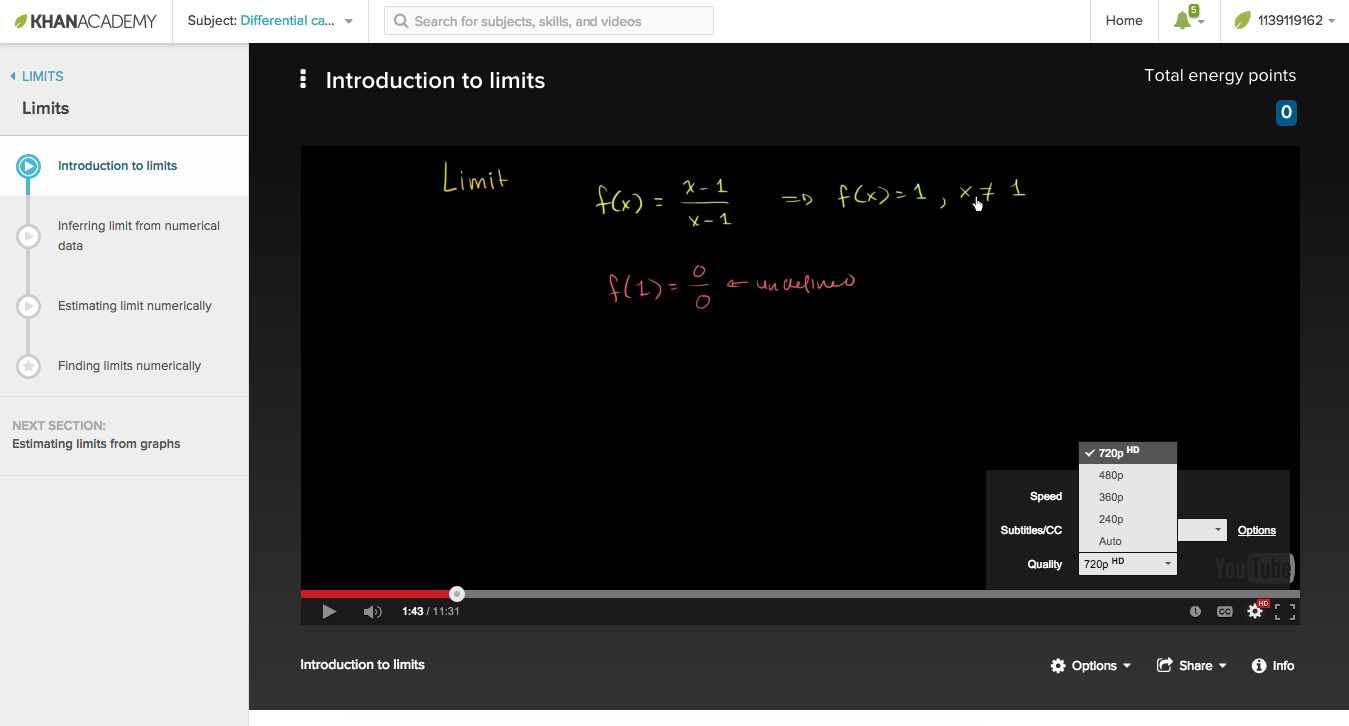
\includegraphics[width=145mm]{../img/khan-academy-screenshot.eps}
		\caption{Khan Academy lesson\label{fig:khan-screen}}		
\end{figure}